
\hzsync{equation}{44}
\hzsync{theorem}{3}

\section{\trEnergySurface{}上的\trPeriodicOrbit}
\label{sec:periodic-orbits-energy-surfaces}

我们将要简略描述的这个存在性问题，起源于对\trCelestialMechanics{}中%
\trPeriodicSolution{}的探寻；并且，正如我们将在第 4 章看到的，它还与一些%
特殊的\trSymplecticInvariant{}相关联。为简单起见，我们考虑%
\textbf{\trStandard\trSymplecticManifold}（standard symplectic manifold）%
$(\R^{2n},\omega_{0})$。我们已经看到，一个函数 $H:\R^{2n}\to\R$ 连同%
$\omega_{0}$ 一起，按下式确定了 $\R^{2n}$ 上的\trHamiltonianVectorField{} $X_{H}$：
\begin{equation}\label{eq:ixh-omega0}
i_{X_{H}}\omega_{0}=-dH.
\end{equation}
\trVectorField{} $X_{H}$ 的\trFlow{} $\varphi^{t}$ 使函数 $H$ 保持不变，即
\begin{equation}\label{eq:H-invariant-flow}
H\bigl(\varphi^{t}(x)\bigr)=H(x),\qquad x\in\R^{2n}
\end{equation}
对\trFlow{}有定义的一切 $t$ 都成立，因而 $H$ 是 $X_{H}$ 的一个\textbf{\trFirstIntegral}（first integral）。事实上，%
利用\trFlow{}的定义，对 \eqref{eq:H-invariant-flow} 求导我们便得到
\begin{align*}
\frac{d}{dt}H\bigl(\varphi^{t}\bigr) &= dH\bigl(\varphi^{t}\bigr)\cdot\frac{d}{dt}\varphi^{t}
= dH\bigl(\varphi^{t}\bigr)\cdot X_{H}\bigl(\varphi^{t}\bigr)\\
&= -\omega_{0}\bigl(X_{H},X_{H}\bigr)\circ\bigl(\varphi^{t}\bigr),
\end{align*}
由于 $\omega_{0}$ 是\trAntisymmetric{}的，上式为零。从几何上看，%
\textbf{\trLevelSet}（level set）
\[
S=\bigl\{\,x\in\R^{2n}\ \bigm|\ H(x)=\mathrm{const}\,\bigr\}\subset\R^{2n}
\]
在 $X_{H}$ 的\trFlow{}下是不变的。现在我们假设 $S$ 是一个%
\textbf{\trCompact\trRegular\trEnergySurface}（compact regular energy surface），即
\begin{equation}\label{eq:regular-energy-surface}
dH(x)\neq0\quad\text{对}\quad x\in S.
\end{equation}
于是 $S$ 是一个\trSmooth\trHypersurface，即 $\R^{2n}$ 中一个%
\textbf{\trCodimension}（codimension）为 $1$ 的\textbf{\trSubmanifold}（submanifold），%
它在点 $x\in S$ 处的\trTangentSpace{}由
\[
T_{x}S=\bigl\{\,v\in T_{x}\R^{2n}\ \bigm|\ dH(x)v=0\,\bigr\}.
\]
给出。

\noindent\begin{minipage}{\linewidth}
\centering
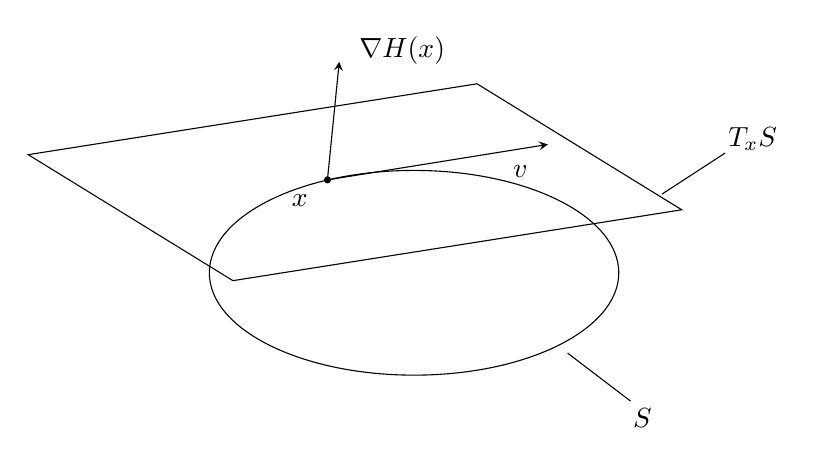
\begin{tikzpicture}[>=stealth]
  \draw (0,0) ellipse (2.6 and 1.3);%
  \draw (-2.3,-0.1) -- (3.4,0.8) -- (0.8,2.4) -- (-4.9,1.5) -- cycle;%
  \fill (-1.1,1.18) circle (1.3pt);%
  \node at (-1.45,0.92) {$x$};
  \draw[->] (-1.1,1.18) -- (1.7,1.63);%
  \node at (1.35,1.28) {$v$};
  \draw[->] (-1.1,1.18) -- (-0.95,2.68);%
  \node at (-0.15,2.82) {$\nabla H(x)$};
  \node at (4.3,1.7) {$T_{x}S$};
  \draw (3.95,1.52) -- (3.15,1.0);%
  \node at (2.9,-1.85) {$S$};
  \draw (2.75,-1.63) -- (1.95,-1.02);%
\end{tikzpicture}

图 1.1
\end{minipage}

显然，对 $x\in S$ 有 $X_{H}(x)\in T_{x}S$，因为%
$dH(x)\cdot X_{H}(x)=-\omega_{0}\bigl(X_{H}(x),X_{H}(x)\bigr)=0$，%
从而 $X_{H}$ 在 $S$ 上定义了一个处处非零的\trVectorField。由于 $S$ 是\trCompact{}的，%
$S$ 上的\trFlow{} $\varphi^{t}$ 对一切时刻都存在。应当强调，%
由于\trHamiltonianVectorField{}所描述的是没有摩擦、振荡永不衰减的系统，%
这个\trFlow{}一般而言是极其复杂的。然而，由于%
\textbf{\trHamiltonianFlow}（Hamiltonian flow）的\trVolumePreserving{}特征，%
$S$ 上的\trFlow{}具有很强的\trRecurrence{}性质。我们将简略回顾这一现象，%
它早已为 H.~\trPoincare{}所知。

设 $\Omega=\omega_{0}\wedge\dots\wedge\omega_{0}$ 为 $\R^{2n}$ 上的\trVolumeForm。%
由于在 $S$ 的一个\trNeighborhood{} $U$ 内 $dH(x)\neq0$，%
我们可以在 $U$ 上找到一个 $(2n-1)$-形式 $\alpha$ 满足
\begin{equation}\label{eq:Omega-dH-alpha}
\Omega=dH\wedge\alpha\qquad\text{在 $U$ 上}.
\end{equation}
记\textbf{包含\trMapping}（inclusion mapping）为 $j:S\to\R^{2n}$，%
则 $(2n-1)$-形式
\begin{equation}\label{eq:mu-pullback}
\mu=j^{*}\alpha\qquad\text{在 $S$ 上}
\end{equation}
显然是 $S$ 上的一个\trVolumeForm。它由 \eqref{eq:Omega-dH-alpha} 唯一确定。%
事实上，若 $\Omega=dH\wedge\alpha=dH\wedge\beta$，则 $dH\wedge(\alpha-\beta)=0$，%
从而对 $U$ 上某个 $(2n-2)$-形式 $\gamma$ 有 $\alpha-\beta=dH\wedge\gamma$。%
鉴于 $j^{*}dH=0$，我们得到 $j^{*}\alpha=j^{*}\beta+j^{*}(dH\wedge\gamma)=j^{*}\beta$，%
正如所断言的。\trVolumeForm{} $\mu$ 在 $X_{H}$ 的\trFlow{} $\varphi^{t}$ 下不变：
\begin{equation}\label{eq:mu-invariant}
\bigl(\varphi^{t}\bigr)^{*}\mu=\mu.
\end{equation}
这由 $\bigl(\varphi^{t}\bigr)^{*}\Omega=\Omega$ 与 $\bigl(\varphi^{t}\bigr)^{*}dH=dH$ 得出。%
事实上，由 \eqref{eq:Omega-dH-alpha} 我们先有 $\Omega=dH\wedge\bigl(\varphi^{t}\bigr)^{*}\alpha$，%
再利用唯一性便得出 $j^{*}\bigl(\varphi^{t}\bigr)^{*}\alpha=j^{*}\alpha$。%
而 $\varphi^{t}\circ j=j\circ\varphi^{t}$，故 $\bigl(\varphi^{t}\bigr)^{*}\bigl(j^{*}\alpha\bigr)=j^{*}\alpha$，%
断言 \eqref{eq:mu-invariant} 得证。若把 $S$ 上由形式 $\mu$ 给出的%
\textbf{\trRegular\trMeasure}（regular measure）记作 $m$，我们看到
\begin{equation}\label{eq:measure-invariance}
m\bigl(\varphi^{t}(A)\bigr)=m(A),\qquad A\subset S.
\end{equation}
此外，$m(S)<\infty$，因为 $S$ 是\trCompact{}的。

\begin{theorem}[\trPoincare{}\trRecurrence{}定理]\label{thm:poincare-recurrence}
设 $S$ 是\trHamiltonianVectorField{} $X_{H}$ 的一个%
\trCompact\trRegular\trEnergySurface，其\trFlow{}为 $\varphi^{t}$。那么 $S$ 上%
\trAlmostEvery{}的点（相对于 $m$）都是\textbf{\trRecurrence{}点}（recurrent point），%
即对几乎每一点 $x\in S$，存在序列 $t_{j}\uparrow\infty$ 满足
\[
\lim_{j\to\infty}\varphi^{t_{j}}(x)=x.
\]
\end{theorem}
\begin{proof}
这个证明出人意料地容易。我们用 $\varphi$ 表示\trFlow{} $\varphi^{t}$ 的%
时刻 $1$ \trMapping。我们首先利用\trMeasure{}的%
\textbf{\trInvariance}（invariance）与有限性证明：对每个 $A\subset S$，
\begin{equation}\label{eq:recurrence-set}
m\Bigl(A\cap\Bigl[\,\bigcap_{k\geq0}\ \bigcup_{j\geq k}\varphi^{-j}(A)\Bigr]\Bigr)=m(A).
\end{equation}
注意，上式方括号 $[\,\cdot\,]$ 中的点，正是那些具有如下性质的点 $x\in S$：%
对每个整数 $k$ 都存在整数 $j\geq k$，使得 $x\in\varphi^{-j}(A)$，%
即 $\varphi^{j}(x)\in A$；它与 $A$ 的交则由 $A$ 中那些无穷多次返回集合 $A$ 的点组成。%
为证明 \eqref{eq:recurrence-set}，我们简记
\[
A_{k}:=\bigcup_{j\geq k}\varphi^{-j}(A),\qquad k=0,1,2,\dots
\]
于是得到子集的递减序列 $A_{0}\supset A_{1}\supset A_{2}\supset\dots$。%
显然 $\varphi^{k}(A_{k})=A_{0}$，从而由 $\varphi$ 保持\trMeasure{}可知 $m(A_{k})=m(A_{0})$。%
由于 $m(A_{0})<\infty$，我们得出：对 $k=0,1,2,\dots$，$A_{0}=A_{k}$ \trAlmostEverywhere{}成立，%
从而 $\bigcap_{k\geq0}A_{k}=A_{0}$ \trAlmostEverywhere{}成立。于是，鉴于 $A\subset A_{0}$，我们得到
\[
A\cap\bigcap_{k\geq0}A_{k}=A\cap A_{0}=A\qquad\text{\trAlmostEverywhere},
\]
这正是所要的等式 \eqref{eq:recurrence-set}。现在我们利用%
\textbf{\trTopology}（topology）中的一个基本事实：$S$ 中存在%
\textbf{\trCountable{}基}（countable basis）。对每个 $n$，都有\trCountable{}多枚半径为%
$\tfrac{1}{n}$ 的\textbf{开\trBall}（open ball）$B_{j}(\tfrac{1}{n})$ 覆盖 $S$。%
把第一步应用到每个\trBall{}上，我们便找到一个\trMeasureZero{}集 $N\subset S$，%
它使得每个 $x\in S\setminus N$ 都无穷多次返回它所属的每个\trBall{}。%
由于对每个 $n$ 都存在 $j=j(x)$ 使 $x\in B_{j}(\tfrac{1}{n})$，定理得证。
\end{proof}

我们指出，\textbf{\trCompactness}（compactness）在此并非实质性要求：%
只要 $S$ 上的\textbf{\trInvariantMeasure}（invariant measure）有限，%
并且 $S$ 的\trTopology{}具有\trCountable{}基，所述结论便成立。正是这一观察使%
\trPoincare{}得以把他的定理应用于\textbf{\trRestrictedThreeBodyProblem}（restricted
three-body problem）。

鉴于\trRecurrence{}定理，在 $S$ 上寻找\trPeriodic{}现象似乎颇为自然。%
人们可以指望，通过对\trHamiltonianSystem{}稍加\trPerturbation，某些\trRecurrence{}点%
不仅会无穷多次返回，而且会在有限时间内\trClosing{}起来，从而产生一个\trPeriodicOrbit。%
这就是所谓的\trClosing{}问题（closing problem）。在其著名的\trClosingLemma{}中，%
C.C.~\trPugh{}与 C.~\trRobinson（[179]，1983）证明了：就\trHamiltonianFunction{}的\emph{$C^{2}$ 范畴}而言，%
\trPeriodicOrbit{}在\trCompact\trRegular\trEnergySurface{}上是\trGeneric\trDense{}的。%
与这种\trGeneric{}现象形成鲜明对照，我们关心的是如下整体存在性问题：

\noindent\textbf{问题：}$(\R^{2n},\omega_{0})$ 中的一个\trCompact\trRegular%
\trEnergySurface{} $S$ 是否具有\trHamiltonianVectorField{} $X_{H}$ 的一个\trPeriodicSolution？

这个问题至今悬而未决。应当强调，我们寻找的是 $S$ 上一个非常受限的%
\trVectorField{}类的\trPeriodicSolution；不妨回顾，H.~\trSeifert（[193]，1950）%
曾提出如下问题：$S^{3}$ 上每个处处非零的\trVectorField{}是否必有%
\textbf{\trClosed\trOrbit}（closed orbit）？这一问题多年悬而未决。%
1974 年，P.A.~\trSchweitzer{} [192] 在 $S^{3}$ 上构造了一个令人惊讶的%
$C^{1}$ 类\trVectorField，它没有任何\trPeriodicSolution；直到很晚近的 1993 年，%
K.~\trKuperberg{} [132] 才给出了 $S^{3}$ 上没有\trPeriodicSolution{}的%
$C^{\infty}$ \trVectorField{}的例子。对于维数高于三维的%
\trManifold{}，同样的问题已于 1966 年由 F.W.~\trWilson{} [228]%
以类似的方式给出了回答。人们还可以问：在更受限的\trMeasurePreserving{}的%
\trSmooth\trVectorField{}类中，是否也会有不含任何\trPeriodicSolution{}的%
\trVectorField。然而，对于\trReeb\trVectorField{}这一特殊类，%
\trClosed\trOrbit{}的存在性晚近已由 H.~\trHofer{} [118] 所确立：%
$S^{3}$ 上每个\trSmooth\trReeb\trVectorField{}都具有一个\trPeriodicOrbit。%
若在 $S^{3}$ 上存在一个\trOneForm{} $\lambda$，使得 $\lambda\wedge d\lambda$%
定义一个\trVolumeForm，且
\[
i_{X}d\lambda=0\quad\text{与}\quad i_{X}\lambda=1,
\]
则称 $S^{3}$ 上的\trVectorField{} $X$ 为\trReeb\trVectorField。我们将在第 4 章中%
结合\textbf{\trContact\trManifold}（contact manifold）上的\trWeinstein{}猜想，%
再回到\trReeb\trVectorField。

后文中至关紧要的一点是：上述问题不依赖于表示 $S$ 的那个%
\trHamiltonianFunction{}的特殊选取，它只依赖于这个\trHypersurface{}与%
\trSymplecticStructure。这一事实是众所周知的，%
它早已见于\trCelestialMechanics{}的\textbf{\trTwoBodyProblem}（two-body problem）中%
\textbf{\trCollision\trSingularity}（collision singularity）的\textbf{\trRegularization}（regularization）之中。%
设 $F$ 是定义 $S$ 的第二个函数，满足
\begin{equation}\label{eq:two-defining-functions}
S=\bigl\{\,x\ \bigm|\ H(x)=c\,\bigr\}=\bigl\{\,x\ \bigm|\ F(x)=c'\,\bigr\}
\end{equation}
且在 $S$ 上 $dH\neq0$，$dF\neq0$。于是 $\ker dF(x)=\ker dH(x)$，%
从而对每个 $x\in S$ 有 $dF(x)=\rho(x)dH(x)$，其中 $\rho$ 是一个处处非零的%
\trSmooth{}函数。因此，这两个\trHamiltonianVectorField{}是平行的：
\begin{equation}\label{eq:parallel-vector-fields}
X_{F}=\rho X_{H}\qquad\text{在 $S$ 上},
\end{equation}
其中 $\rho(x)\neq0$。由此可见，$X_{H}$ 与 $X_{F}$ 在 $S$ 上具有相同的\trOrbit，%
尽管一般而言二者的\textbf{\trParametrization}（parametrization）互不相同。更确切地说，若 $\varphi^{t}$ 是 $X_{H}$ 在 $S$ 上的%
\trFlow，则 $X_{F}$ 在 $S$ 上的\trFlow{} $\psi^{s}$ 由下式给出：
\begin{equation}\label{eq:flow-reparametrization}
\psi^{s}(x)=\varphi^{t}(x),\qquad t=t(s,x),\qquad x\in S,
\end{equation}
其中函数 $t$ 由\trDifferentialEquation
\[
\frac{dt}{ds}=\rho\bigl(\varphi^{t}(x)\bigr),\qquad t(0,x)=0,
\]
所定义，它依赖于参数 $x\in S$。我们看到，特别地，$X_{H}$ 与 $X_{F}$ 具有相同的%
\trPeriodicOrbit。

例如，设 $X_{H}$ 具有\trEnergySurface{}%
$S=\bigl\{\,x\in\R^{2n}\ \bigm|\ \tfrac{1}{2}|x|^{2}=R>0\,\bigr\}$，%
则 $X_{H}$ 在 $S$ 上的一切解都是\trPeriodic{}的。事实上，%
由 $F(x)=\tfrac{1}{2}|x|^{2}$ 定义的\trHamiltonianFunction{} $F$ 同样把%
$S=\bigl\{\,x\ \bigm|\ F(x)=R\,\bigr\}$ 表示为一个\trRegular\trEnergySurface。%
\trVectorField{} $X_{F}$ 是\trLinear{}的，其\trFlow{}为
\[
\psi^{s}(x)=e^{sJ}x=(\cos s)x+(\sin s)Jx,
\]
它显然是\trPeriodic{}的。

我们可以用一个特定的\textbf{\trLineBundle}（line bundle）把问题更抽象地重新表述。%
设 $S$ 是 $\R^{2n}$ 中的一个\trHypersurface。于是 $T_{x}S$ 的维数为 $2n-1$，%
从而 $\omega_{0}$ 限制到 $T_{x}S$ 上必定是\trDegenerate{}的，且%
\textbf{\trRank}（rank）为 $(2n-2)$。因此它的\trKernel{}是 $1$ 维的；我们看到，%
$\omega_{0}$ 与 $S$ 一起确定了\trLineBundle
\begin{equation}\label{eq:characteristic-line-bundle}
\mathcal{L}_{S}=\bigl\{\,(x,\xi)\in TS\ \bigm|\ \omega_{0}(\xi,v)=0\quad\text{对一切}\quad v\in T_{x}S\,\bigr\}.
\end{equation}
若 $S$ 是 $X_{H}$ 的一个\trRegular\trEnergySurface，则对一切 $v\in T_{x}S$ 有%
$\omega_{0}\bigl(X_{H}(x),v\bigr)=-dH(x)v=0$。于是，
\[
X_{H}(x)\in\mathcal{L}_{S}(x),\qquad x\in S
\]
对每一个以 $S$ 为\trRegular\trEnergySurface{}的\trHamiltonianVectorField{}都成立。%
于是，$X_{H}$ 在 $S$ 上的\trPeriodicSolution{}对应于\trLineBundle{}%
$\mathcal{L}_{S}$ 的\trClosedCharacteristic；%
后者定义为 $S$ 中的一维\trSubmanifold{} $P\subset S$，它\trDiffeomorphism{}于\textbf{\trCircle}（circle），%
其各\trTangentSpace{}属于 $\mathcal{L}_{S}$，即 $TP=\mathcal{L}_{S}|P$。于是，%
\trRegular\trEnergySurface{}上\trHamiltonianEquation{}的\trPeriodicSolution{}%
存在性问题可以几何地重述如下：

\noindent\textbf{问题：}$(\R^{2n},\omega_{0})$ 中的一个%
\trCompact\trSmooth\trHypersurface{} $S$ 是否容有特定\trLineBundle{}%
$\mathcal{L}_{S}$ 的一条\trClosedCharacteristic？

注意，$\mathcal{L}_{S}$ 由\trHypersurface{}与 $\omega_{0}$ 所定义。第 4 章将证明：%
存在\trHypersurface{} $S\subset\R^{2n}$ 以及 $S$ 附近异于 $\omega_{0}$ 的%
\trSymplecticStructure{} $\omega$，使得 $S$ 相对于 $\omega$ 的\trLineBundle{}%
不容有\trClosedCharacteristic。

这一整体存在性问题的突破归功于 A.~\trWeinstein{} [225] 与%
P.~\trRabinowitz{} [181]\footnote{原书印作「[225]」，与同句 A.~\trWeinstein{}之引注同号；然 [225] 实系 A.~\trWeinstein{}之文献，而 P.~\trRabinowitz{}此文在原书文献表中编号为 [181]，原书第 4 章引用此文亦作 [181]，此处径改。——译者注}：他们在 1978 年分别在 $\R^{2n}$ 中的%
\trConvex\trHypersurface{}与\textbf{\trStarShaped\trHypersurface}（star-like
hypersurface）上建立了\trClosedCharacteristic{}的存在性。这些证明以%
\textbf{\trVariationalPrinciple}（variational principle）为基础。特别是，%
P.~\trRabinowitz{}证明：先前曾被用于推导\trHamiltonianVectorField{}之形式变换性质的%
那条高度\trDegenerate{}的\trAction{}原理，可以十分有效地用于存在性证明。%
这一关键思想在其后的发展中被证明是决定性的；在这一发展中，下一个里程碑是%
C.~\trViterbo{}于 1987 年对 $\R^{2n}$ 中 A.~\trWeinstein{}猜想的证明。该猜想断言：%
每一个\textbf{\trContactType\trHypersurface}（hypersurface of contact type）%
都具有一个\trClosedCharacteristic。这类在\trSymplectic{}意义下受限制的\trHypersurface{}将在第 4 章中描述，%
该章专门讨论\trSymplecticManifold{}中\trHypersurface{}上%
\trClosedCharacteristic{}的存在性。我们应当提到，每个\trCompact\trHypersurface{} $S$%
都会产生大量的\trPeriodicOrbit；然而这些\trOrbit{}未必位于给定\trSurface{}上，%
而是位于邻近的\trSurface{}上。我们用一个结果来说明这一点，该结果也将在第 4 章中得到证明。%
设\trHypersurface{} $S$ 属于由
\[
S_{\varepsilon}=\bigl\{\,x\ \bigm|\ H(x)=1+\varepsilon\,\bigr\}\subset\R^{2n}
\]
所定义的族，其中 $\varepsilon$ 取遍以 $0$ 为中心的一个区间 $I$ 内的值，而 $S$ 对应于 $S_{0}$。

\begin{theorem}\label{thm:almost-every-epsilon}
对几乎每个 $\varepsilon\in I$，$\R^{2n}$ 中的\trHypersurface{} $S_{\varepsilon}$%
都具有\trHamiltonianVectorField{} $X_{H}$ 的一个\trPeriodicSolution。
\end{theorem}

在第 4 章中，我们将从一个特定的\trSymplecticInvariant{}出发，%
轻而易举地推出这一现象。
